\chapter{Documentation Standards}\label{record-005}

\noindent{\footnotesize\color{BookMuted}\path{docs/DOCUMENTATION_STANDARDS.md}\par}\smallskip

\textbf{Status:} Current project policy for new and substantially changed documentation.

\textbf{Applies to:} User, DOGFOOD, component, CLI, MCP, runtime, IR, release, workflow, and contributor documentation in Bijou.

\textbf{Normative terms:} \textbf{MUST}, \textbf{SHOULD}, and \textbf{MAY} indicate requirement strength.

This standard adapts reader-task documentation discipline to Bijou's existing contract and DOGFOOD practices. It does not require a mass rewrite of existing pages. Apply it when creating documentation, changing behavior, or touching a page enough that leaving it below this bar would create new debt.

\section{1. Purpose}\label{record-005-purpose}

Documentation is part of the product contract. A Bijou page should help a specific reader do one of these jobs:

\begin{itemize}
\tightlist
\item
  learn the product through a guided first success;
\item
  complete a real task in their own environment;
\item
  look up exact facts while working;
\item
  understand a concept, invariant, boundary, or design choice;
\item
  troubleshoot an observable failure;
\item
  change the implementation safely and verify the result;
\item
  inspect a release, cycle, or architecture decision and its evidence.
\end{itemize}

A page MUST have one primary job. Do not force a README, design document, topic page, or release packet to behave as a tutorial, reference manual, roadmap, and architecture guide at the same time.

\section{2. Corpus Map}\label{record-005-corpus-map}

Bijou keeps durable truth in a small set of known places.

\begin{center}
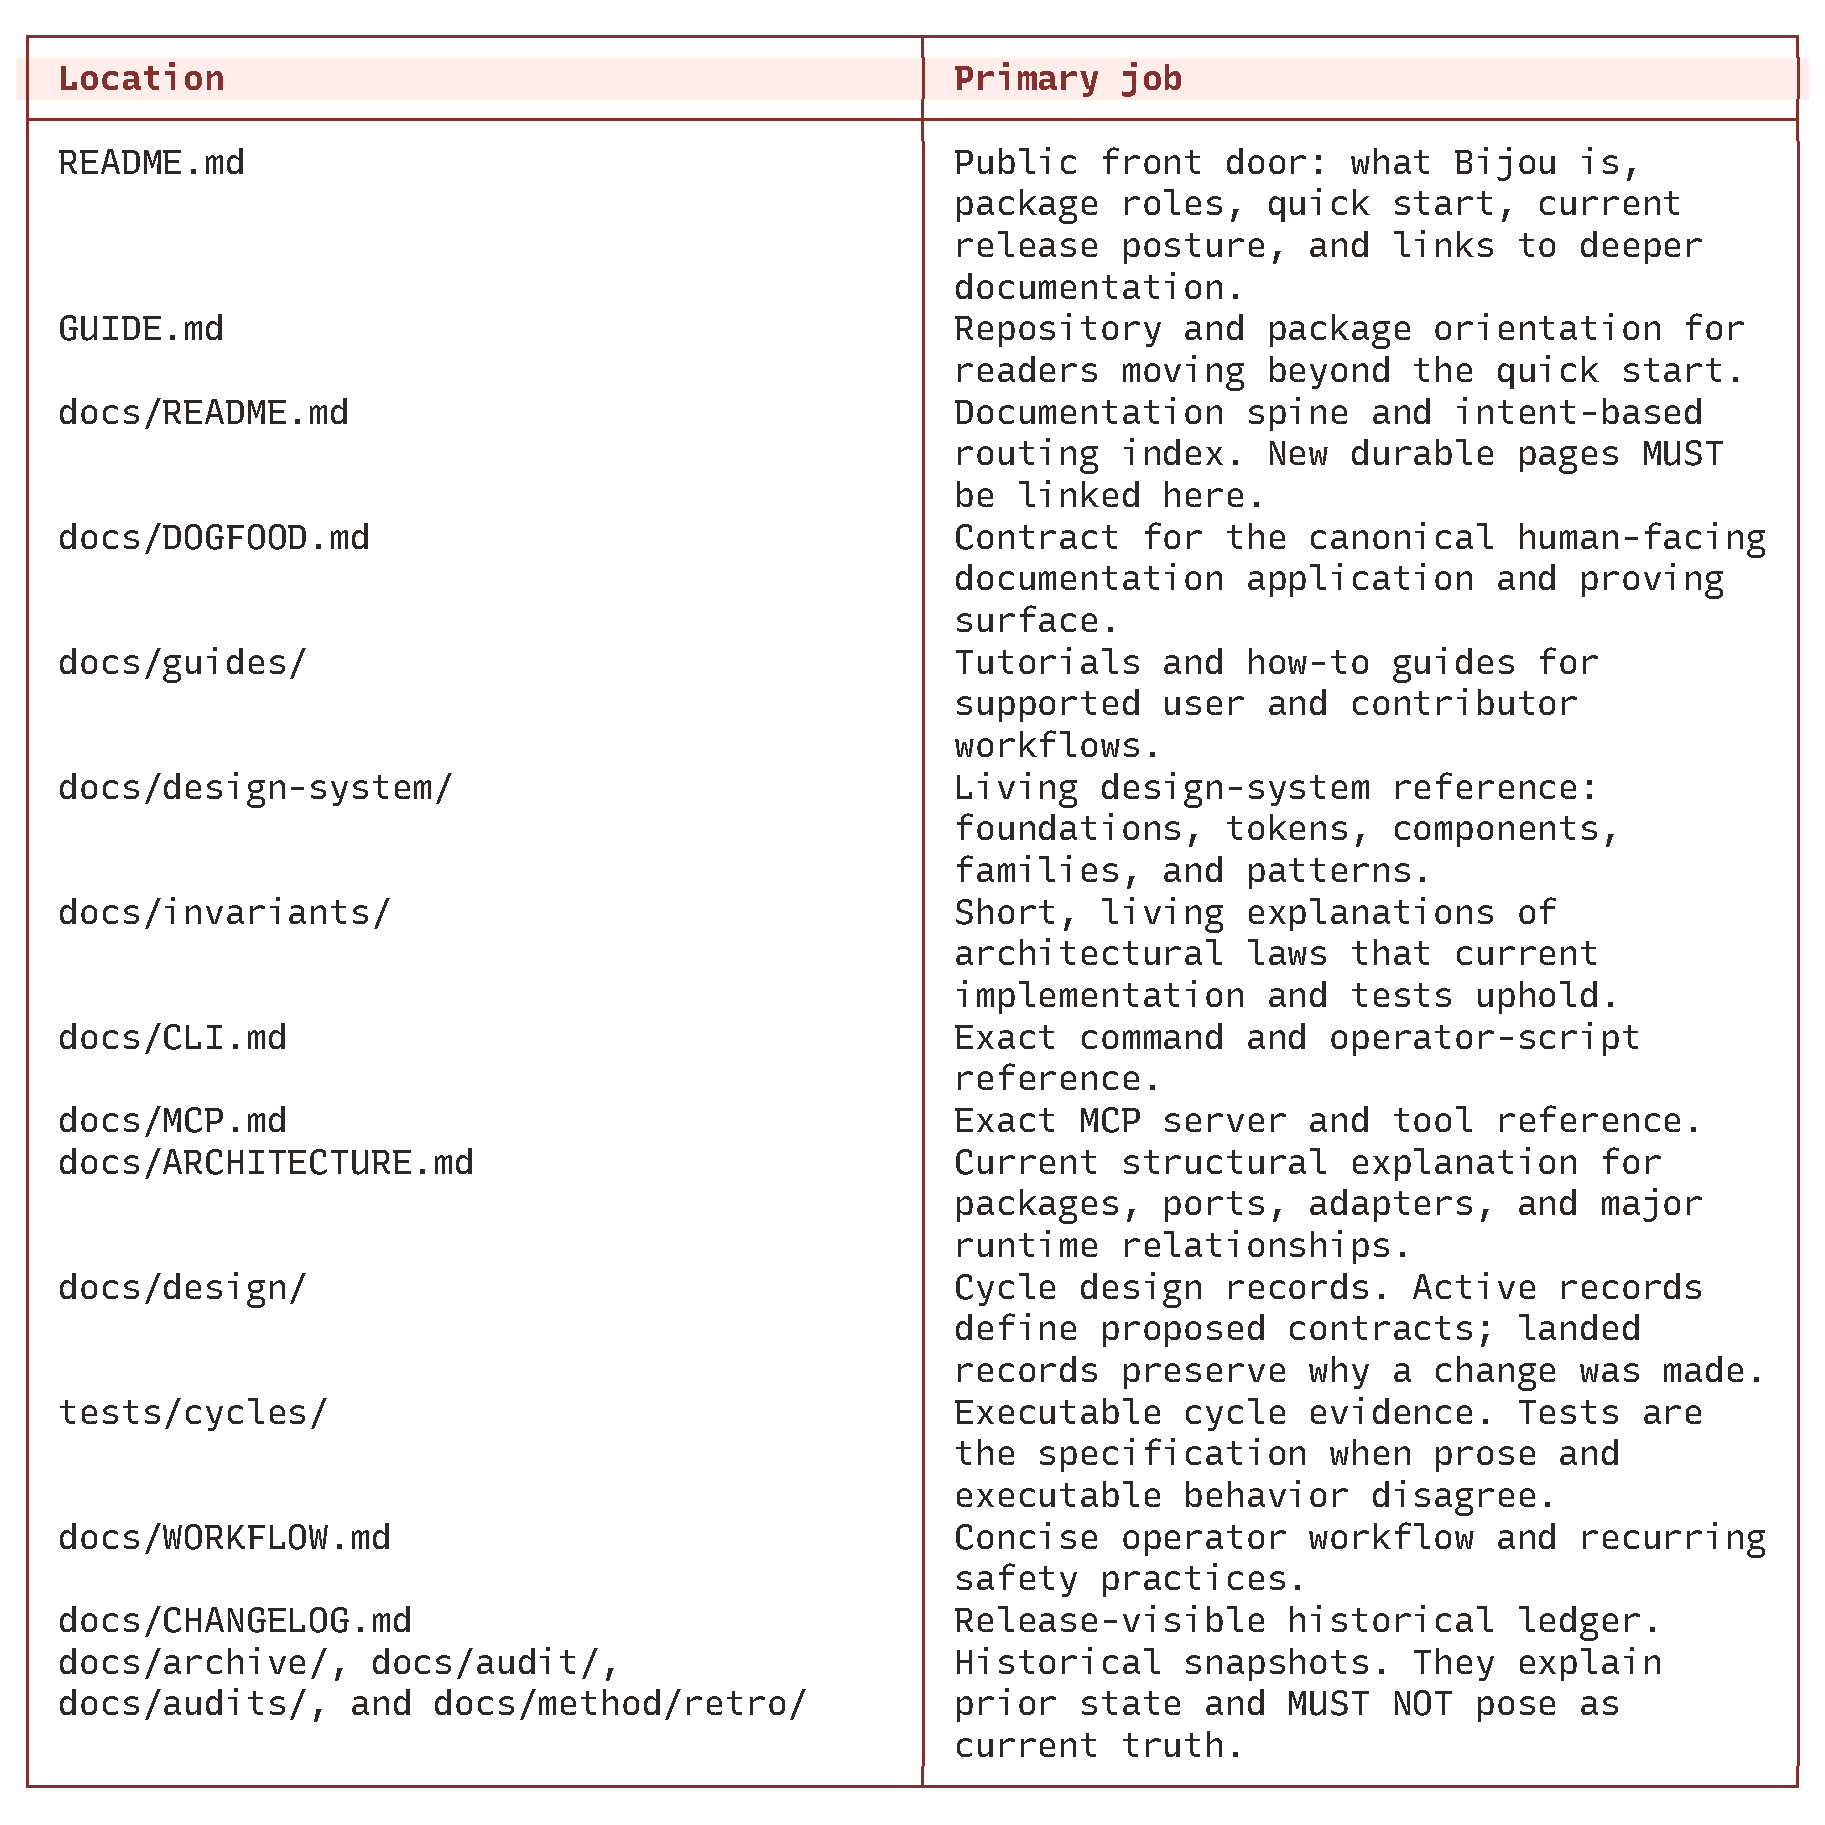
\includegraphics[width=\linewidth]{figures/tables/table-007-g1-1.pdf}
\par\smallskip{\scriptsize\color{BookMuted}Rows 1–15. Actual Bijou table component.}
\end{center}


GitHub issues and milestones own roadmap and release scope. Linear is the chosen execution tracker; migration is pending connection and workspace/team selection. Until verified Linear links exist, source GitHub issues remain live. Repository documentation explains contracts, decisions, and evidence, not mirrored queue state.

Do not create empty placeholder directories. Add a page when it has a real reader job.

\section{3. Page Types}\label{record-005-page-types}

\subsection{3.1 Tutorial}\label{record-005-tutorial}

A tutorial is a guided learning path. Use one when a newcomer needs a controlled first success, such as rendering a first component or building a small framed application.

A tutorial MUST:

\begin{itemize}
\tightlist
\item
  state prerequisites and starting state;
\item
  use a known-good supported path;
\item
  provide actions in tested order;
\item
  show expected intermediate and final results;
\item
  explain how to verify success;
\item
  end with what the reader learned and where to go next.
\end{itemize}

\subsection{3.2 How-To Guide}\label{record-005-how-to-guide}

A how-to guide helps a competent reader complete a real task, such as adding a component to DOGFOOD, recording a fixture, or running a release gate.

A how-to guide MUST:

\begin{itemize}
\tightlist
\item
  be titled as a goal, preferably starting with a verb;
\item
  state the expected result;
\item
  identify blocking prerequisites;
\item
  give the shortest safe route to the result;
\item
  include exact commands, settings, controls, or API calls;
\item
  explain how to verify success;
\item
  link to reference or explanation instead of reproducing it.
\end{itemize}

\subsection{3.3 Reference}\label{record-005-reference}

Reference pages support exact lookup. Public reference includes:

\begin{itemize}
\tightlist
\item
  package exports and component options;
\item
  CLI commands, arguments, exit behavior, and output;
\item
  MCP tools, inputs, results, and errors;
\item
  IR, artifact, source-map, receipt, and validation contracts;
\item
  theme tokens, component families, and lower-mode behavior;
\item
  configuration, environment variables, and repository scripts.
\end{itemize}

Reference MUST state exact names, syntax, fields, defaults, constraints, compatibility behavior, output, errors, and examples. When the underlying surface is machine-readable, reference SHOULD be generated or coverage checked.

Reference describes behavior that exists. Proposed behavior belongs in a design record, issue, or roadmap.

\subsection{3.4 Explanation And Invariant}\label{record-005-explanation-and-invariant}

Explanation develops a mental model: why Bijou separates Components from Blocks, why layout owns interaction geometry, or why graceful lowering preserves meaning.

Explanation SHOULD describe mechanisms, relationships, tradeoffs, alternatives, and limits. It MUST NOT become an unstructured source-file tour.

An invariant page states one durable law. It MUST name:

\begin{itemize}
\tightlist
\item
  the law;
\item
  the boundary it protects;
\item
  observable consequences;
\item
  executable evidence or the current evidence gap.
\end{itemize}

\subsection{3.5 Design Record}\label{record-005-design-record}

A design record shapes one bounded change. It MUST identify:

\begin{itemize}
\tightlist
\item
  the decision summary and hill;
\item
  current truth;
\item
  scope and non-goals;
\item
  public, runtime, artifact, or workflow contract;
\item
  tests to write first;
\item
  acceptance criteria;
\item
  playback questions;
\item
  tracker ownership.
\end{itemize}

Proposed work is not evidence. After implementation, the record SHOULD include the measured result or link to its witness.

\subsection{3.6 Test Plan And Executable Evidence}\label{record-005-test-plan-and-executable-evidence}

A test plan is the contract ledger for behavior. It MUST identify:

\begin{itemize}
\tightlist
\item
  stable requirement or cycle identities where the repository uses them;
\item
  planned or implemented cases;
\item
  the exact behavior or invariant under test;
\item
  the oracle;
\item
  the evidence type;
\item
  the status;
\item
  the concrete test, fixture, script, or witness when implemented.
\end{itemize}

A gap MUST be marked as a gap. Planned work MUST NOT be described as passing evidence.

\subsection{3.7 Troubleshooting}\label{record-005-troubleshooting}

Troubleshooting starts with a symptom a user or operator can observe, such as:

\begin{itemize}
\tightlist
\item
  terminal output is missing color;
\item
  input reaches the wrong layer;
\item
  DOGFOOD does not render;
\item
  an artifact fails validation;
\item
  a release or Code Dojo gate fails.
\end{itemize}

A troubleshooting page MUST list discriminating checks first, map signals to likely causes, give concrete recovery actions, and show how to verify the fix.

\subsection{3.8 Workflow Reference}\label{record-005-workflow-reference}

A workflow reference describes a recurring contributor or maintainer operation, such as preparing a release, processing review feedback, or updating a ratchet.

A workflow reference MUST:

\begin{itemize}
\tightlist
\item
  describe only the current operational contract;
\item
  identify authoritative scripts and runbooks;
\item
  link to workflow verification or witness evidence;
\item
  place warnings before destructive, privileged, or externally visible steps;
\item
  avoid duplicating product reference, release notes, or roadmap promises.
\end{itemize}

\subsection{3.9 Release And Historical Record}\label{record-005-release-and-historical-record}

A release packet records a bounded release decision, its scope, gates, and publication evidence. A changelog records notable user- or operator-visible change.

Historical records MUST remain clearly historical. Do not silently rewrite a past audit, retro, or shipped release record to match current implementation. Add a current reference or a dated correction instead.

\section{4. Documentation Upkeep Loop}\label{record-005-documentation-upkeep-loop}

For a meaningful behavior, contract, or workflow change:

\begin{enumerate}
\def\labelenumi{\arabic{enumi}.}
\tightlist
\item
  Update design or rationale when the change needs design discussion.
\item
  Update the relevant test plan or cycle contract before implementation.
\item
  Add the smallest deterministic executable evidence that fails for the missing behavior.
\item
  Implement the behavior.
\item
  Update living reference after the behavior exists.
\item
  Mark planned cases implemented and record the actual evidence.
\item
  Update \texttt{R\allowbreak{}E\allowbreak{}A\allowbreak{}D\allowbreak{}M\allowbreak{}E\allowbreak{}.\allowbreak{}m\allowbreak{}d}, \texttt{d\allowbreak{}o\allowbreak{}c\allowbreak{}s\allowbreak{}/\allowbreak{}R\allowbreak{}E\allowbreak{}A\allowbreak{}D\allowbreak{}M\allowbreak{}E\allowbreak{}.\allowbreak{}m\allowbreak{}d}, \texttt{d\allowbreak{}o\allowbreak{}c\allowbreak{}s\allowbreak{}/\allowbreak{}C\allowbreak{}H\allowbreak{}A\allowbreak{}N\allowbreak{}G\allowbreak{}E\allowbreak{}L\allowbreak{}O\allowbreak{}G\allowbreak{}.\allowbreak{}m\allowbreak{}d}, the external tracker when public surface, documentation routing, release status, or project posture changes.
\item
  Run documentation upkeep before final self-review and before requesting final pull-request review.
\end{enumerate}

Small fixes may scale this down. They still need an honest claim, executable evidence when behavior changes, and living documentation that does not contradict the result.

\section{5. Examples And Executable Truth}\label{record-005-examples-and-executable-truth}

Examples are part of the contract.

User-facing examples MUST:

\begin{itemize}
\tightlist
\item
  be syntactically valid;
\item
  use supported behavior;
\item
  include enough context to run or interpret them;
\item
  use least-privileged and safe defaults;
\item
  identify destructive or privileged actions before they appear;
\item
  show an observable result when one exists.
\end{itemize}

Examples SHOULD be extracted from tested files or executed in CI when practical.

\subsection{5.1 Runnable, Illustrative, And Abridged Examples}\label{record-005-runnable-illustrative-and-abridged-examples}

A runnable example uses supported behavior and includes required context. Test or execute it automatically when practical.

An illustrative example may omit setup or nonessential detail, but it MUST be labeled illustrative and MUST NOT be presented as directly runnable.

An abridged example may shorten large input or output, but it MUST identify the omitted material and preserve the behavior relevant to the explanation.

\subsection{5.2 Code Blocks And Terminal Examples}\label{record-005-code-blocks-and-terminal-examples}

Every fenced block SHOULD declare its language or content type:

\begin{itemize}
\tightlist
\item
  \texttt{b\allowbreak{}a\allowbreak{}s\allowbreak{}h} or \texttt{s\allowbreak{}h} for copyable shell commands;
\item
  \texttt{t\allowbreak{}y\allowbreak{}p\allowbreak{}e\allowbreak{}s\allowbreak{}c\allowbreak{}r\allowbreak{}i\allowbreak{}p\allowbreak{}t}, \texttt{j\allowbreak{}s\allowbreak{}o\allowbreak{}n}, \texttt{y\allowbreak{}a\allowbreak{}m\allowbreak{}l}, or the relevant language for structured input;
\item
  \texttt{t\allowbreak{}e\allowbreak{}x\allowbreak{}t} for expected output;
\item
  \texttt{c\allowbreak{}o\allowbreak{}n\allowbreak{}s\allowbreak{}o\allowbreak{}l\allowbreak{}e} only for a deliberate transcript containing prompts and output.
\end{itemize}

Do not include \texttt{\$} or \texttt{>} prompts in a block intended for copy and paste. Present commands and output separately.

Run:

\begin{CodeBlock}
npm run code-dojo:debt
\end{CodeBlock}

Expected output shape:

\begin{CodeBlock}
Code Dojo debt: N violations
\end{CodeBlock}

When output is nondeterministic, say which parts vary. Label output as exact, representative, or abridged when the distinction matters. Never fabricate output to make an example appear complete.

\subsection{5.3 Placeholders}\label{record-005-placeholders}

Use clearly fictional and context-safe values.

\begin{center}
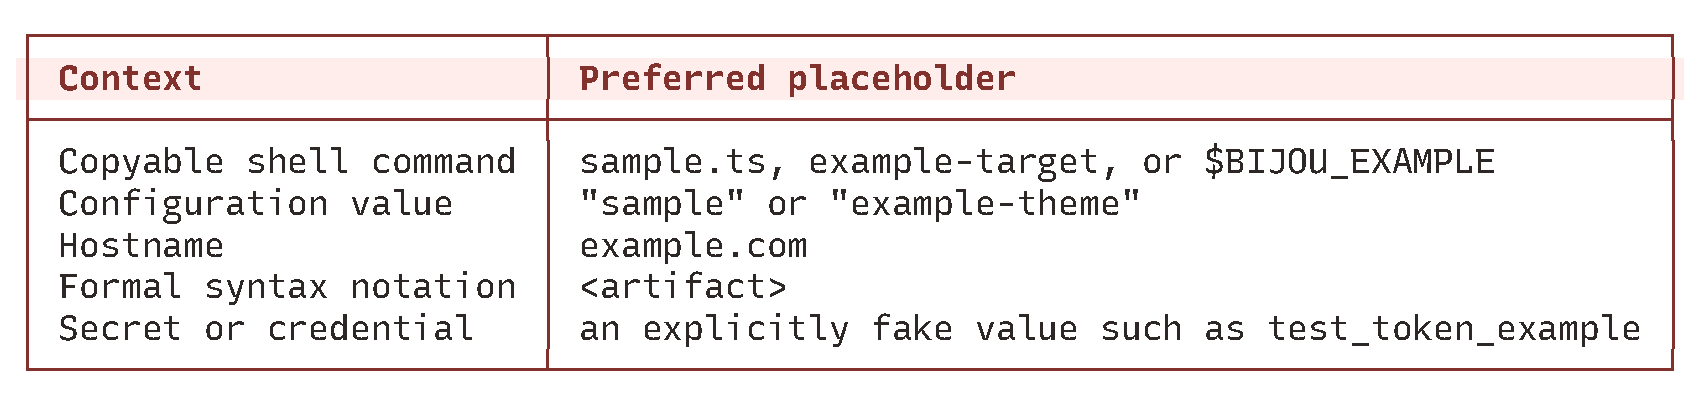
\includegraphics[width=\linewidth]{figures/tables/table-008-g1-1.pdf}
\par\smallskip{\scriptsize\color{BookMuted}Rows 1–5. Actual Bijou table component.}
\end{center}


Do not use \texttt{<\allowbreak{}y\allowbreak{}o\allowbreak{}u\allowbreak{}r\allowbreak{}-\allowbreak{}f\allowbreak{}i\allowbreak{}l\allowbreak{}e\allowbreak{}>} inside a copyable shell command because angle brackets have shell meaning.

\subsection{5.4 Dangerous Commands}\label{record-005-dangerous-commands}

For destructive, privileged, costly, irreversible, or externally visible actions:

\begin{enumerate}
\def\labelenumi{\arabic{enumi}.}
\tightlist
\item
  Place the warning before the command.
\item
  State the exact consequence and scope.
\item
  Provide a dry run or safer alternative when available.
\item
  State required permissions.
\item
  Include backup or rollback guidance when applicable.
\item
  Explain how to verify the result.
\end{enumerate}

\section{6. Visuals And Accessibility}\label{record-005-visuals-and-accessibility}

Visual products should be shown visually when the visual answers a reader question. Bijou documentation MAY use terminal captures, DOGFOOD fixtures, screenshots, annotated examples, or short recordings.

Every nontrivial visual MUST:

\begin{itemize}
\tightlist
\item
  answer a stated or obvious reader question;
\item
  have meaningful labels or adjacent explanation;
\item
  include alt text or a concise textual equivalent;
\item
  distinguish conceptual simplification from exact implementation when needed;
\item
  omit secrets, personal data, production identifiers, and sensitive details.
\end{itemize}

Informative images MUST have alt text or a textual equivalent. Decorative images SHOULD have empty alt text where the publishing surface supports it. Complex diagrams SHOULD have adjacent explanatory prose instead of relying on a long alt attribute.

Visuals MUST NOT rely on color, position, animation, or shape alone to communicate essential meaning. Screenshots and recordings MUST NOT be the only place where essential instructions, code, or errors appear.

Terminal examples MUST preserve accessible and pipe-mode meaning when the document claims those modes are supported.

\section{7. Writing, Style, And Terminology}\label{record-005-writing-style-and-terminology}

Write like a competent teammate: direct, precise, and approachable.

\begin{itemize}
\tightlist
\item
  Use \texttt{y\allowbreak{}o\allowbreak{}u} for actions the reader performs.
\item
  Use \texttt{B\allowbreak{}i\allowbreak{}j\allowbreak{}o\allowbreak{}u}, the package name, command, script, or component name for actions the system performs.
\item
  Use imperative verbs for procedures.
\item
  Prefer active voice when it clarifies responsibility.
\item
  Use present tense for current behavior.
\item
  Avoid hype, vague reassurance, unnecessary apology, and excessive exclamation.
\item
  Avoid \texttt{w\allowbreak{}e} unless referring to an explicit project decision or policy.
\end{itemize}

Put the result, decision, warning, or essential condition first. Give each sentence one main job. Use numbered lists for ordered procedures and bullets for parallel options, requirements, or checks.

\subsection{7.1 Markdown And Typography}\label{record-005-markdown-and-typography}

Use formatting to communicate type, not to manufacture emphasis.

\begin{itemize}
\tightlist
\item
  Use bold for exact visible labels and genuine warnings.
\item
  Use inline code for commands, options, filenames, paths, configuration keys, fields, literal values, error identities, and code symbols.
\item
  Use exact casing for products, packages, commands, fields, and errors.
\item
  Use \texttt{<\allowbreak{}k\allowbreak{}b\allowbreak{}d\allowbreak{}>} for keyboard keys where the publishing surface renders it accessibly; otherwise use inline code.
\item
  Use descriptive link text that states what the destination provides.
\item
  Do not use \texttt{h\allowbreak{}e\allowbreak{}r\allowbreak{}e}, \texttt{t\allowbreak{}h\allowbreak{}i\allowbreak{}s\allowbreak{} \allowbreak{}l\allowbreak{}i\allowbreak{}n\allowbreak{}k}, or a bare filename as the entire link label.
\item
  Declare a language or content type on fenced blocks.
\end{itemize}

Use tables only for genuinely two-dimensional lookup, comparison, or structured facts. Do not use them for long narrative passages or procedures.

\subsection{7.2 Canonical Terminology}\label{record-005-canonical-terminology}

Use one canonical term for each concept. Define unfamiliar terms at first use. Mention an alias once only when it materially improves search or recognition.

Use exact Bijou distinctions:

\begin{itemize}
\tightlist
\item
  A \textbf{Component} is leaf rendering vocabulary.
\item
  A \textbf{Block} owns product semantics, data contracts, and lowering facts.
\item
  A \textbf{Surface} is structured terminal-cell output.
\item
  \texttt{u\allowbreak{}i\allowbreak{}-\allowbreak{}s\allowbreak{}c\allowbreak{}e\allowbreak{}n\allowbreak{}e\allowbreak{}-\allowbreak{}i\allowbreak{}r\allowbreak{}/\allowbreak{}1}, \texttt{b\allowbreak{}i\allowbreak{}j\allowbreak{}o\allowbreak{}u\allowbreak{}-\allowbreak{}b\allowbreak{}l\allowbreak{}o\allowbreak{}c\allowbreak{}k\allowbreak{}/\allowbreak{}1}, and other versioned artifacts are explicit contracts.
\item
  Interactive, static, pipe, and accessible are output modes with distinct claims.
\item
  A command requests change; an effect interacts with the outside world.
\end{itemize}

\subsection{7.3 Inclusive And Accessible Language}\label{record-005-inclusive-and-accessible-language}

Use literal, neutral language that describes the technical condition directly.

\begin{itemize}
\tightlist
\item
  Use gender-neutral language when gender is irrelevant.
\item
  Avoid identity-based or stigmatizing metaphors.
\item
  Prefer unavailable, hidden, degraded, unresponsive, excluded, or blocked when those are the actual conditions.
\item
  Avoid culturally specific idioms when they make instructions harder to understand or translate.
\end{itemize}

\subsection{7.4 Notes, Cautions, And Warnings}\label{record-005-notes-cautions-and-warnings}

Use callouts consistently:

\begin{itemize}
\tightlist
\item
  \textbf{Note} --- useful context that does not affect safety or correctness.
\item
  \textbf{Important} --- information required to complete the task correctly.
\item
  \textbf{Caution} --- an action may cause an undesirable or costly result.
\item
  \textbf{Warning} --- an action may cause data loss, a security problem, or an irreversible change.
\end{itemize}

Do not use a warning merely to make ordinary text look important.

\section{8. Checks And Enforcement}\label{record-005-checks-and-enforcement}

Documentation quality requires deterministic checks and human judgment.

Run the current repository documentation gates for documentation changes:

\begin{CodeBlock}
npm run docs:inventory
git diff --check
\end{CodeBlock}

When design-system documentation changes, also run:

\begin{CodeBlock}
npm run docs:design-system:preflight
\end{CodeBlock}

When workflow files change, run an available pinned workflow validator. If the repository does not provide one, record that absence rather than claiming the workflow was validated.

The repository contains \texttt{.\allowbreak{}m\allowbreak{}a\allowbreak{}r\allowbreak{}k\allowbreak{}d\allowbreak{}o\allowbreak{}w\allowbreak{}n\allowbreak{}l\allowbreak{}i\allowbreak{}n\allowbreak{}t\allowbreak{}.\allowbreak{}j\allowbreak{}s\allowbreak{}o\allowbreak{}n}, but no pinned Markdown-lint runner or internal-link checker is currently part of \texttt{p\allowbreak{}a\allowbreak{}c\allowbreak{}k\allowbreak{}a\allowbreak{}g\allowbreak{}e\allowbreak{}.\allowbreak{}j\allowbreak{}s\allowbreak{}o\allowbreak{}n}. Until those tools land, Markdown style and internal links remain required review checks rather than falsely reported automated gates.

CI SHOULD block on facts it can determine reliably:

\begin{itemize}
\tightlist
\item
  malformed Markdown when a pinned checker exists;
\item
  broken internal paths and explicit anchors when an offline checker exists;
\item
  references to repository files that do not exist;
\item
  failed examples or tutorials declared executable;
\item
  undocumented public commands, options, settings, fields, statuses, or errors when coverage is required;
\item
  informative images without alt text or a textual equivalent;
\item
  changed contract behavior without updated evidence or a documented no-documentation-impact decision;
\item
  destructive examples without a preceding warning;
\item
  examples containing real credentials or forbidden production identifiers.
\end{itemize}

The following SHOULD normally remain advisory:

\begin{itemize}
\tightlist
\item
  page, sentence, or paragraph length;
\item
  passive voice and jargon density;
\item
  number of bullets;
\item
  suspected missing diagrams;
\item
  tone and template-like phrasing;
\item
  table complexity;
\item
  external-link health;
\item
  screenshot age;
\item
  pull-request size.
\end{itemize}

These signals help editors. They are poor universal merge gates.

\section{9. Review Checklist}\label{record-005-review-checklist}

Before calling a documentation change complete, check:

\begin{itemize}
\tightlist
\item
  The page has one primary reader job.
\item
  Living references describe the behavior proposed for the merge target.
\item
  Planned work lives in a design record, test plan, roadmap, issue, or PR.
\item
  Examples use supported behavior and show observable results when practical.
\item
  Public commands, options, settings, fields, statuses, and errors have or link to reference coverage.
\item
  User-facing terminal behavior has a capture, fixture, or textual equivalent when a visual materially helps.
\item
  New durable pages are linked from \texttt{d\allowbreak{}o\allowbreak{}c\allowbreak{}s\allowbreak{}/\allowbreak{}R\allowbreak{}E\allowbreak{}A\allowbreak{}D\allowbreak{}M\allowbreak{}E\allowbreak{}.\allowbreak{}m\allowbreak{}d}.
\item
  Release-visible changes update \texttt{d\allowbreak{}o\allowbreak{}c\allowbreak{}s\allowbreak{}/\allowbreak{}C\allowbreak{}H\allowbreak{}A\allowbreak{}N\allowbreak{}G\allowbreak{}E\allowbreak{}L\allowbreak{}O\allowbreak{}G\allowbreak{}.\allowbreak{}m\allowbreak{}d}.
\item
  Direction or release-order changes update GitHub issues and milestones, with linked Linear execution items once connected.
\item
  \texttt{n\allowbreak{}p\allowbreak{}m\allowbreak{} \allowbreak{}r\allowbreak{}u\allowbreak{}n\allowbreak{} \allowbreak{}d\allowbreak{}o\allowbreak{}c\allowbreak{}s\allowbreak{}:\allowbreak{}i\allowbreak{}n\allowbreak{}v\allowbreak{}e\allowbreak{}n\allowbreak{}t\allowbreak{}o\allowbreak{}r\allowbreak{}y} and \texttt{g\allowbreak{}i\allowbreak{}t\allowbreak{} \allowbreak{}d\allowbreak{}i\allowbreak{}f\allowbreak{}f\allowbreak{} \allowbreak{}-\allowbreak{}-\allowbreak{}c\allowbreak{}h\allowbreak{}e\allowbreak{}c\allowbreak{}k} pass.
\end{itemize}

The objective is not a perfectly uniform library. The objective is a documentation corpus where readers, reviewers, tests, and agents can find the right authoritative page at the moment they need it.

